\setchapterpreamble[u]{\margintoc}
\chapter{Phenomenology of TeV Neutrinos}
\labch{nu_theory}

The concept of the neutrino, initially called the "neutron," was first proposed by Pauli in 1930 \sidecite{Pauli} to explain the observed continuous energy spectrum in the beta decay process. Even 60 years after the first direct detection of neutrinos from nuclear reactors by Cowan and Reines \sidecite{nu_discovery}, neutrinos are still the subject of intense experimental investigation, and many of their fundamental properties remain to be measured. This chapter details fundamental properties of Neutrinos in standard model, their interactions and other properties. Last section shall highlight properties and interactions assuming theories \emph{Beyond Standard Model}.

\section{Neutrinos in Standard Model}
\label{sec:sm_nu}
In the Standard Model (SM) of particle physics, neutrinos are fundamental particles characterized as massless, chargeless, and colorless fermions that come in three distinct flavors: electron neutrinos ($\nu_e$), muon neutrinos ($\nu_\mu$), and tau neutrinos ($\nu_\tau$). Neutrinos interact solely via the weak force, which is mediated by the exchange of $W^\pm$ and $Z^0$ bosons, making them highly elusive and difficult to detect in experiments. This weak interaction is responsible for the rare instances where neutrinos can interact with other particles, allowing them to traverse vast distances across the universe almost unhindered. The Standard Model is built upon the conservation of charge, parity, and time reversal symmetry (\emph{CPT symmetry}). Under CPT symmetry, for every left-handed fermion, there exists a corresponding right-handed antiparticle with an opposite charge. However, this symmetry does not necessitate the existence of a right-handed particle state. In the case of neutrinos, the SM originally postulated them as Weyl fermions—particles that have no mass and possess only left-handed components. Consequently, the left-handed neutrino was considered the particle, and the right-handed antineutrino its antiparticle. 


\subsection{Mass and Oscillations}
\label{sec:nu_mass_osc}
The Standard model neutrinos were initially thought to be massless, but when the Homestake experiment measured the flux of solar neutrinos (electron anti-neutrinos ($\bar{\nu}_e$)) \sidecite{homestake}, which was one third of what the solar models predicted \sidecite{Bethe39}, many theories of neutrino oscillations\footnote{Technically, this in itself hints towards Physics beyond standard model as in order for neutrinos to oscillate between flavours, at least two of the three flavours must have non-zero mass.} were put forward to explain why the deficit was observed. The Sudbury Neutrino Observatory later confirmed neutrino oscillations by detecting all neutrino flavors through neutral-current interactions \sidecite{Ahmad_2001}, aligning with solar models. Additional confirmation came from the Super-Kamiokande detector measurement, which observed the disappearance of atmospheric muon neutrinos after passing through the Earth \sidecite{SuperK_osc}, further substantiating neutrino oscillations. 

The weak interactions violate parity symmetry, as shown by Chien-Shiung Wu in 1956 through her study of the beta decay of cobalt-60 nuclei \sidecite{Wu}. This discovery revealed that only left-handed particles and right-handed antiparticles take part in weak interactions, violating CPT symmetry. This finding also raised the possibility that neutrinos might have right-handed particles and left-handed antiparticles, but they are not observed due to the weak interaction's non-preference. In the Standard Model, fermions acquire mass through interactions with the Higgs field, which requires both left-handed and right-handed states. However, no right-handed neutrinos have been observed, leading to speculation about how neutrinos obtain their mass. One possible explanation is the introduction of a right-handed neutrino that interacts with the Higgs field, resulting in \textbf{Dirac neutrinos}, which maintain lepton number conservation. Alternatively, the right-handed state could be identified as the antiparticle of the left-handed state, leading to \textbf{Majorana neutrinos}, where the neutrino is its own antiparticle, without imposing lepton number conservation.

Although oscillations have confirmed that neutrinos are not massless, the precise values are still uncertain, with only upper limits currently known. Direct measurements derived from the beta decay energy spectrum indicate that the effective electron neutrino mass is likely less than 0.8eV \sidecite{katrin}. Indirect astrophysical and cosmological observations provide an even more stringent constraint, suggesting that the sum of all neutrino masses ($\sum{{m}_{\nu}})$ is below 0.12 eV \sidecite{cosmologymass}. 

\subsubsection*{Neutrino Oscillations in Vacuum}
\label{sec:nu_osc_vacuum}
It was first suggested by Bruno Pontecorvo that neutrino oscillations would be possible if neutrinos had mass \sidecite{Pontecorvo}. In accordance with this theory, when a neutrino is produced in a weak interaction, it is in a flavor eigenstate denoted as $\nu_{\alpha}$. However, this flavor eigenstate is actually a superposition of the neutrino mass eigenstates $\nu_{i}$, which are the true eigenstates of the Hamiltonian governing neutrino propagation. Mathematically, the flavor eigenstate $\nu_{\alpha}$ can be expressed as:
\begin{equation}\label{eq:flav_to_mass}
        |\nu_{\alpha}\rangle = \sum_{j=1}^{N_{\nu}} U_{\alpha j}^* |\nu_j\rangle
\end{equation}
\marginnote{
        \begin{kaobox}
        The number of active neutrinos, denoted as $N_{\nu}$, is determined to be 3 based on experimental observations. This was done by measuring the decay width of the $Z^0$ boson at LEP using electron-positron collisions at the resonance energy of the $Z^0$ particle \cite{Z_decay}. The result, $N_{\nu} = 2.984\pm  0.008$, is consistent with the existing understanding of 3 active neutrino flavors. 
        \end{kaobox}}
where, where $N_{\nu}$  represents the number of neutrino species, here assumed to be 3 \sidecite{Z_decay}, and $U$ is the Pontecorvo-Maki-Nakagawa-Sakata (PMNS) mixing matrix (analogous to CKM Matrix in quark sector). This matrix encapsulates the probabilities of different mass eigenstates contributing to a particular flavor eigenstate. 
The PMNS mixing matrix $U^*$ can be written as a product of rotation matrices and phase factors:

\begin{equation*}\label{eq:pmns}
U^{*} = \begin{pmatrix}
1 & 0 & 0 \\
0 & c_{23} & s_{23} \\
0 & -s_{23} & c_{23} 
\end{pmatrix}
\begin{pmatrix}
c_{13} & 0 & s_{13} e^{i\delta} \\
0 & 1 & 0 \\
-s_{13} e^{i\delta} & 0 & c_{13} 
\end{pmatrix}
\begin{pmatrix}
c_{12} & s_{12} & 0 \\
-s_{12} & c_{12} & 0 \\
0 & 0 & 1
\end{pmatrix}
\begin{pmatrix}
e^{i\alpha_1} & 0 & 0 \\
0 & e^{i\alpha_2} & 0 \\
0 & 0 & 1
\end{pmatrix},
\end{equation*}

where $c_{ij} = \cos\theta_{ij}$ and $s_{ij} = \sin\theta_{ij}$ represent the mixing angles between different neutrino flavors, $\delta$ is the Dirac CP-violating phase, and $\alpha_1$ and $\alpha_2$ are the Majorana phases. These parameters control the extent and nature of neutrino mixing, ultimately determining how likely a neutrino produced as one flavor is to be detected as another after propagating a certain distance. The mixing parameters of the matrix have been extensively measured through various experiments, including studies of atmospheric neutrinos in IceCube \sidecite{IceCube_atm_numixing}. The latest fit-results of a global fit (NuFIT 5.3) \sidecite{Esteban:2020cvm} using data of many experiments is shown in \reftab{mixing_parameters}. While the values of $\Delta m^2_{ij}$ are well determined, the sign of the mass-squared difference is only known for $\Delta m^2_{12}$, resulting in two possible mass orderings. In the normal ordering (NO), the masses follow $m_1 < m_2 < m_3$, while in the inverted ordering (IO), the hierarchy is $m_3 < m_1 < m_2$. The data indicate that the strongest mixing occurs between $\nu_1$ and $\nu_2$, as well as between $\nu_2$ and $\nu_3$. The mass ordering and the CP-violating phase $\delta_{\text{CP}}$ remain largely unconstrained, but recent global fits suggest a preference for $\delta_{\text{CP}} \neq 0$ and indicate that the normal ordering is favored over the inverted ordering.

\begin{table}[h!]
        \caption{The oscillation parameters determined from the NuFIT 5.3 (2024) global analysis \cite{Esteban:2020cvm}. Results are presented for the assumption of a normal mass hierarchy and an inverted mass hierarchy. Here $\Delta m^2_{3l}$ represents $\Delta m^2_{31}$ for the normal hierarchy or $\Delta m^2_{32}$ for the inverted hierarchy. The parameters are shown for globalfit values without SuperKamiokande's atmospheric data, for more details see \url{http://www.nu-fit.org}}
        \labtab{mixing_parameters}
        {\renewcommand{\arraystretch}{1.4}
        \begin{tabular}{LLL}
            \hline
            \hline
             & \mathrm{Normal \, Ordering} & \mathrm{Inverted \, Ordering}\\
            \hline
            \theta_{12} [^{\circ}] &33.66_{-0.70}^{+0.73}&33.67_{-0.71}^{+0.73}\\
            \theta_{23} [^{\circ}] &49.1_{-1.3}^{+1}&49.5_{-1.2}^{+0.9}\\
            \theta_{13} [^{\circ}] &8.54_{-0.11}^{+0.11}&8.57_{-0.11}^{+0.11}\\
            \delta_{\mathrm{CP}} [^{\circ}] &197_{-25}^{+41}&286_{-32}^{+27}\\
            \Delta m^2_{21}[10^{-5}\mathrm{eV}^2]&7.41_{-0.20}^{+0.21}&7.41_{-0.20}^{+0.21}\\
            \Delta m^2_{3l}[10^{-5}\mathrm{eV}^2]&+2.51_{-0.027}^{+0.027}&-2.498_{-0.024}^{+0.032}\\
            \hline
            \hline
\end{tabular}}
\end{table}
In addition to the assumed three neutrino species, throughout the remainder of this discussion (as derived in \sidecite{Osc_derivation}) of neutrino oscillation, neutrinos are assumed to be Dirac particles and hence the fourth matrix in Equation \ref{eq:pmns}, containing Majorana Phases is dropped\sidenote{Additionally, throughout the derivation, Natural units are used, i.e $\hbar=c=1$. Hence, mass is in units of energy and time is given in the units of distance.} 

After traveling a distance \(L\) (or, equivalently for relativistic neutrinos, time \(t\)), a neutrino originally produced with a flavor \(\alpha\) evolves as follows:

\begin{equation}\labeq{}
|\nu_\alpha(t)\rangle = \sum_{j=1}^{n} U_{\alpha j}^* |\nu_j(t)\rangle,
\end{equation}

Using an approximation that the neutrino state is a plane wave $|\nu_j(t)\rangle = e^{-iE_j t} |\nu_j(0)\rangle$, and assuming neutrinos are relativistic, The transition probability of a neutrino initially produced with flavour $\nu_{\alpha}$ to $\nu_{\beta}$ after time $t$ can be given as,
\marginnote{
        \begin{kaobox}
        In Equation~\ref{eq:main_probability}, the term $\frac{\Delta m_{jk}^2 L}{2E}$ is a replacement for $(E_j-E_k)t$. In ultra-relativistic limits, if all mass eigenstates have the same momentum, one can approximately express the energy in terms of the mass of each state as,
        \begin{equation}\label{eq:mass_limit}
                E_j = \sqrt{p_j^2 + m_j^2} \approx E + \frac{m_j^2}{2E}.
                \end{equation}
         Also, by assuming all neutrinos are travelling approximately at the speed of light $c$, time $t$ can be expressed in terms of propagation length $L$.
        \end{kaobox}}
\begin{equation}\label{eq:oscillation}
        \begin{split}
                P(\nu_\alpha \rightarrow \nu_\beta) &= |\langle \nu_\beta | \nu_\alpha(t) \rangle|^2 \\
                &=  \sum_{j,k} U_{\alpha j}^* U_{\beta j} U_{\alpha k} U_{\beta k}^* e^{-i(E_{j}-E_{k})t} 
        \end{split}
\end{equation}
            

Using the orthogonality relation $\langle \nu_i(0) | \nu_j(0) \rangle = \delta_{ij}$ of the mass eigenstates, the transition probability becomes:

\begin{equation}\label{eq:main_probability}
P(\nu_\alpha \rightarrow \nu_\beta) \approx \sum_{j,k} U_{\alpha j}^* U_{\beta j} U_{\alpha k} U_{\beta k}^* e^{-i \frac{\Delta m_{jk}^2 L}{2E}},
\end{equation}

The mass-squared difference between the mass eigenstates j and k, denoted as $\Delta m_{jk}^2 = m_j^2 - m_k^2$, is calculated as the difference between $m_j^2$ and $m_k^2$. The probability of flavor transition is a periodic function of the distance L between the source and the detector and is influenced by the mass-squared differences and the neutrino energy. 

\marginnote{\begin{kaobox}
        The transition probability derived in Equation~\ref{eq:twoflavour_transition} has a period with the oscillation length ($L_{\mathrm{osc}}$) determined by the neutrino energy ($E_{\nu}$) and mass difference ($\Delta m^2$) as,
        \begin{equation}\label{eq:twoflav}
                L_{\mathrm{osc}} = \frac{4 \pi E_{\nu}}{\Delta m^2}
        \end{equation}
        and the amplitude is proportional to the mixing angle. From Equation ~\ref{eq:twoflav} for an experiment to be sensitive to a specific value of $\Delta m^2$, it must be configured so that $E/L \approx \Delta m^2$. For example, to measure the parameters $\theta_{23}$ and $\Delta m^2_{32}$, an $L/E$ value of approximately 500 km/GeV is required, which is typical for atmospheric neutrino studies. To probe the parameters $\theta_{12}$ and $\Delta m^2_{12}$, the appropriate $L/E$ would be around 15,000 km/GeV, as seen in solar neutrino experiments. The distance between the neutrino sources and detector, is usually reffered to as \emph{baseline} of the experiment
\end{kaobox}}

In most scenarios, neutrino oscillations can be approximated by two-flavor mixing due to the suppression of three-flavor mixing effects by the small value of $\theta_{13}$ and the large hierarchy between the two mass-squared splittings, where $\Delta m_{21}^2 \ll \Delta m_{32}^2$. As a result, the problem is often simplified to two-flavor oscillations. The transition probability exhibits an oscillatory behavior, hence the name. If $L \gg L_{\mathrm{osc}}$, the oscillating phase completes many cycles before detection and is averaged to 1/2., \emph{Neutrino Oscillations}.

In the simplest case of two-flavor mixing, the mixing matrix depends on just one mixing angle, and there is only one relevant mass-squared difference. The probability\footnote{The probability is the same for neutrinos and antineutrinos.} that a neutrino $\nu_{\alpha}$ with energy $E_{\nu}$ oscillates into a neutrino $\nu_{\beta}$ after traveling a distance L (the so-called \emph{transition probability}) is given by:

\begin{equation}\label{eq:twoflavour_transition}
P(\nu_\alpha \rightarrow \nu_\beta) = \sin^2(2\theta) \sin^2\left(\frac{\Delta m^2 L}{4 E_\nu}\right), \quad \alpha \neq \beta.
\end{equation}

As opposed to the case where the probability that a neutrino $\nu_{\alpha}$ with energy $E_{\nu}$ after traveling a distance L is still measured in state of $\nu_{\alpha}$ (the so-called \emph{survival probability}) is given by:

\begin{equation}\label{eq:twoflavour_survival}
        P(\nu_\alpha \rightarrow \nu_\alpha) = 1-\sin^2(2\theta) \sin^2\left(\frac{\Delta m^2 L}{4 E_\nu}\right), \quad \alpha = \beta.
\end{equation}

\subsubsection*{Neutrino Oscillations in Matter}
\label{sec:nu_osc_matter}
The discussion so far has assumed that neutrinos travel through a vacuum. However, when neutrinos travel through matter, their interactions with the medium alter their properties. This happens because of coherent forward scattering on electrons and nucleons, which modifies the amplitude of their propagation. Initially the idea that the oscillation parameters of neutrinos are altered in matter was coined by Lincoln Wolfenstein's \sidecite{MSW1,MSW2}. In 1985, Stanislav Mikheyev and Alexei Smirnov predicted that a gradual decrease in the density of matter can resonantly enhance neutrino mixing \sidecite{MSW3}. 

In the presence of matter, the Hamiltonian of the system changes by experiencing an \emph{Effective Potential} ($V_{\mathrm{eff}}$). As a result, the mass eigenstates and eigenvalues of  this effective hamiltonian changes, meaning that neutrinos in matter now have a different effective mass than they did in a vacuum. Since neutrino oscillations depend on the squared mass difference of the neutrinos, neutrino oscillations experience different dynamics than they did in a vacuum. This theory formed basis to solve the solar neutrino puzzle, where observed deficit of neutrino fluxes could only be explained by not only neutrino oscillations but also the matter effects that the produced neutrinos in the sun core goes through while reaching the surface, and later crossing the threshold of higher matter density to vacuum \sidecite{MSW4,MSW5}. 

\subsection{Interactions}
\label{sec:nu_interactions}
In the Standard Model, neutrinos only interact through the weak interaction, which is mediated by the exchange of the $W^{\pm}$ and $Z^0$ bosons. These bosons have masses of $M_{W^{\pm}}=80$ GeV  and $M_{Z^0}=91$ GeV \sidecite{PDG_2024}. The massiveness of these bosons contribute to the weakness of the interaction in normal conditions. Processes involving the W-boson are referred to as charged-current (CC) processes, while those involving the Z-boson are called neutral-current (NC) processes Neutrinos interact with charged leptons ($e^{\pm}$, $\mu^{\pm}$, $\tau^{\pm}$) through scattering processes and are produced in the decays of unstable charged leptons such as $\mu^{\pm}$ and $\tau^{\pm}$. They also interact with quarks, both in bound states (e.g., neutrons, protons, pions) through neutrino-nucleon scattering, and as individual quarks (partons) through deep inelastic scattering

This section will cover the general properties of neutrino interactions, focusing on their cross-sections across various energy scales. Later subsections will explore high-energy interaction processes, which are important for understanding neutrino behavior in extreme environments and are relevant to the analysis presented in this thesis.

\subsubsection*{Interaction Cross-Sections}
\label{sec:xsec}
Neutrino interactions can exhibit a wide range of behaviors \sidecite{xsec_overview} depending on the energy at which they occur and whether the interaction involves a neutrino or an antineutrino, as shown in \reffig{total_xsec}. 

\begin{figure*}[h!]
        \begin{subfigure}[h]{0.7\textwidth}
            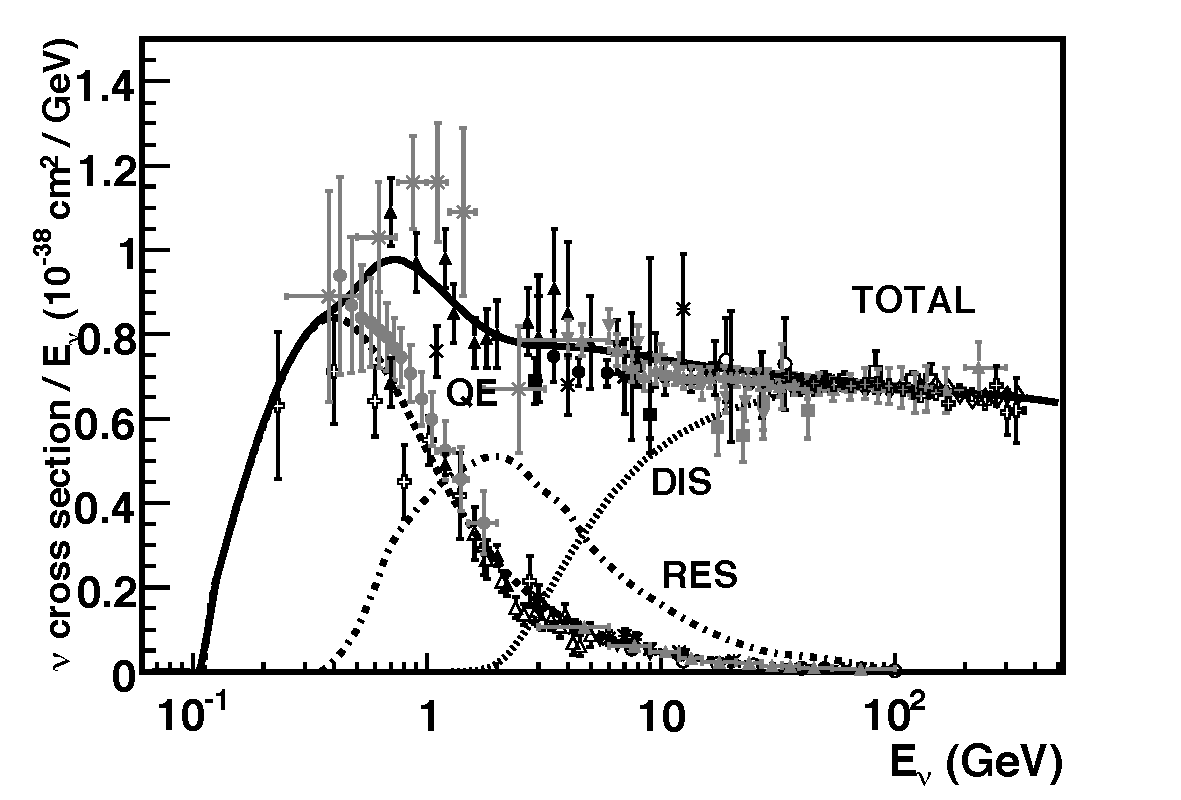
\includegraphics{./figures/nu_phenomenology/cc_inclusive_nu.pdf}
        \end{subfigure}
        \hfill
        \begin{subfigure}[h]{0.7\textwidth}
            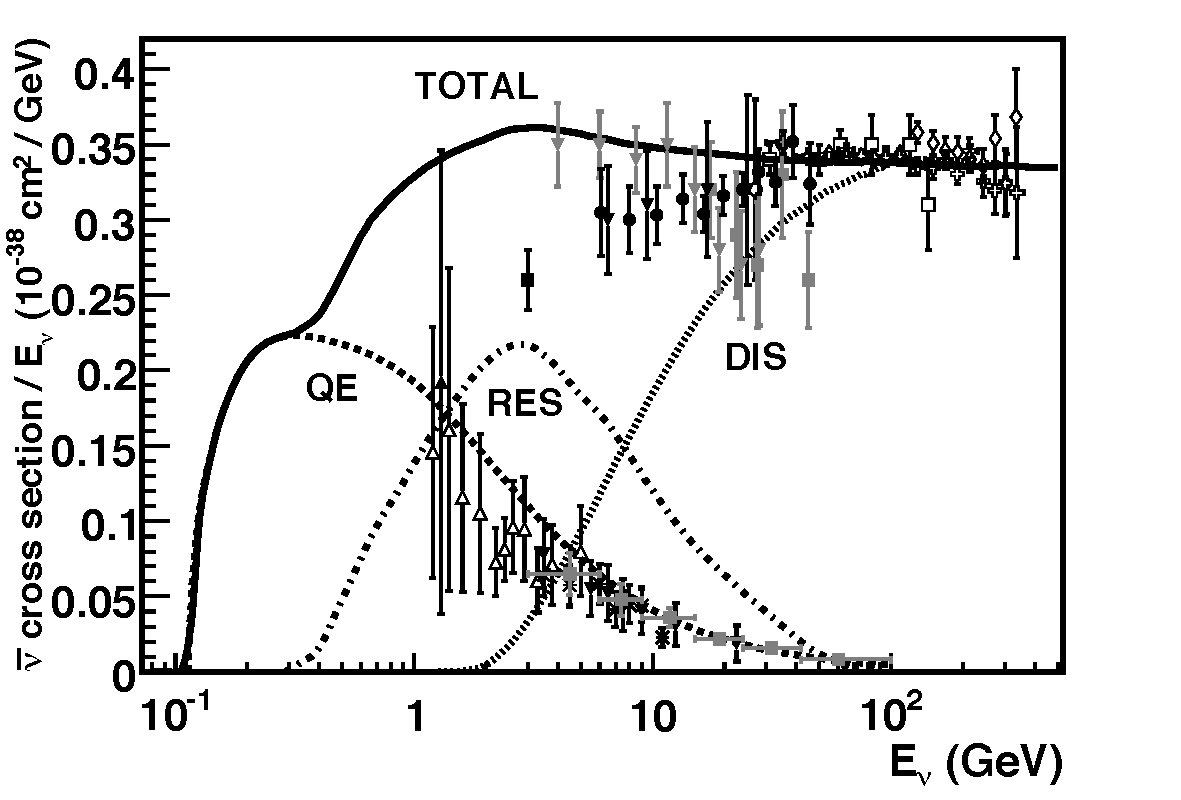
\includegraphics{./figures/nu_phenomenology/cc_inclusive_nubar.pdf}
        \end{subfigure}
        
        \caption{Total cross-sections for neutrinos (left) and antineutrinos (right) per nucleon in charged-current interactions (for an isoscalar target) divided by neutrino energy as a function of neutrino energy. Figure taken from \cite{xsec_overview} }
        \labfig{total_xsec}
\end{figure*}

\marginnote{\begin{kaobox}[title=\textbf{Inverse Beta Decay (IBD)}]
       In IBD, $\bar{\nu_{e}}$ interacts with a proton, producing a $e^+$ and a neutron. The $\bar{\nu_{e}}$ must have a minimum kinetic energy of 1.806 MeV to initiate the reaction. This is due to the mass difference between the reactants and products. The positron receives most of the antineutrino's energy due to its smaller mass compared to the neutron.
        \begin{equation}\label{eq:IBD}
                 \bar{\nu}_e + p \rightarrow e^+ + n 
        \end{equation}
\end{kaobox}
}
At low energies, typically up to around 1 MeV, neutrino interactions are dominated by scattering off leptons and nuclei, both in charged and neutral forms. Two notable processes in this energy range are \textbf{coherent scattering} and \textbf{Neutrino Capture on Radioactive Nuclei}. These low-energy interactions can be described through electroweak theory, where the neutrino engages in two-body scattering processes. As the neutrino energy increases, it becomes possible to probe the target nucleus at progressively smaller length scales. While coherent scattering treats the nucleus as a unified structure, higher-energy neutrinos can resolve individual nucleons. One significant low-energy process is the Inverse Beta Decay (IBD). This process has been extensively studied in several experiments such as KamLAND \sidecite{KamLAND_osc} and Daya Bay \sidecite{DayaBay}, which measures neutrino oscillations using  anti-neutrinos produced in fission nuclear reactors, typically probing energies up to around 10 MeV.

As the energy increases to the GeV range, neutrinos primarily interact through \textbf{quasi-elastic scattering} and \textbf{resonance production}. In quasi-elastic scattering, neutrinos interact with nucleons, producing charged leptons without breaking apart the nucleon. At slightly higher energies, resonance production becomes a crucial interaction mode. In this case, neutrinos excite the target nucleon into resonance states, such as $\Delta$ or $N^*$, which subsequently decay into various final states, yielding combinations of nucleons and mesons. The energy range of around 10 GeV is often called \emph{the transition region} because it separates quasi-elastic scattering, where the target is a nucleon, from \textbf{ the deep inelastic scattering (DIS)}, where the target is a quark (or \emph{parton}) within the nucleon. As shown in \reffig{total_xsec}, above this transition region ($> 100$ GeV), the total cross-section exhibits an almost linear relationship with neutrino energy and DIS becomes the dominant process of all neutrino interactions. This scaling behavior, as predicted by the quark-parton model \sidecite{parton}, assumes point-like scattering off quarks. However, these assumptions are not valid at lower neutrino energies, where lower momentum transfers have a greater impact on the interaction dynamics \sidecite{xsec_overview}. Since this energy range is critical for high-energy neutrino interactions in IceCube, especially for the analysis presented in this thesis, only DIS (and other relavnt processes at this energy, see Section \ref{sec:glashow}) process shall be discussed in more detail. 

\subsubsection*{Neutrino-Nucleon Deep Inelastic Scattering}
\label{sec:DIS}
\begin{marginfigure}
\centering
\begin{tikzpicture}
\begin{feynman}
        \def\flen{1.5}
        \def\boslen{1.4}
        \def\fangle{45}

        
        

        \vertex (v1)  at (0, \boslen);
        \vertex (i1) at ($(v1) + (180-\fangle:\flen)$) {$\barp{\nu_{l}}$};
        \vertex (f1) at ($(v1) + (\fangle:\flen)$) {$\mathcal{l}^{\pm}$};

        \vertex (v2)  at (0, 0) ;
        \vertex (i2) at ($(v2) + (\fangle-180:\flen)$) {$N$};
        \vertex (f2) at ($(v2) + (-\fangle:\flen)$) {$X$};

        \diagram* {
        (i1) -- [fermion] (v1) -- [fermion] (f1),
        (v1) -- [boson, edge label=$W^{\mp}$] (v2),
        (i2) -- [fermion] (v2) -- [fermion] (f2)
        };
\end{feynman}
\end{tikzpicture}
\caption{Feynman diagram of Neutrino-Nucleon DIS via CC interaction.}
\labfig{DIS_CC}
\end{marginfigure}
\begin{marginfigure}
\centering
\begin{tikzpicture}
\begin{feynman}
        \def\flen{1.5}
        \def\boslen{1.4}
        \def\fangle{45}

        % in order to get the [dot] to work, we need to add the empty braces
        

        \vertex (v1) at (0, \boslen);
        \vertex (i1) at ($(v1) + (180-\fangle:\flen)$) {$\barp{\nu_{l}}$};
        \vertex (f1) at ($(v1) + (\fangle:\flen)$) {$N$};

        \vertex (v2) at (0, 0);
        \vertex (i2) at ($(v2) + (\fangle-180:\flen)$) {$\barp{\nu_{l}}$};
        \vertex (f2) at ($(v2) + (-\fangle:\flen)$) {$N'$};

        \diagram* {
        (i1) -- [fermion] (v1) -- [fermion] (f1),
        (v1) -- [boson, edge label=$Z^{0}$] (v2),
        (i2) -- [fermion] (v2) -- [fermion] (f2)
        };
\end{feynman}
\end{tikzpicture}
\caption{Feynman diagram of Neutrino-Nucleon DIS via NC interaction.}
\labfig{DIS_NC}
\end{marginfigure}
In Deep Inelastic Scattering (DIS), neutrinos interact with quarks inside nucleons, breaking them apart and producing a cascade of particles. In this high-energy regime, the neutrino can be seen as scattering off individual partons, but a scattered parton cannot remain free for long. It quickly creates a jet of hadrons through pair production, a process known as hadronization or fragmentation. Both charged-current (CC) and neutral-current (NC) interactions can occur this way, resulting in either an outgoing charged lepton or neutrino. Feynman diagrams of CC and NC interactions for neutrinos are shown in \reffig{DIS_CC} and \reffig{DIS_NC} respectively, with their corresponding reactions in Equation~\ref{eq:CC} and Equation~\ref{eq:NC}. The most general form of the differential neutrino-nucleon cross section for a CC interaction, involving an incoming neutrino with initial four momentum $k_1$, scattering with a target nucleon with four-momentum $p$, resulting in an outgoing lepton with four-momentum $k_2$, and a virtual gauge boson with four-momentum transfer q=$k_1-k_2$, can be expressed as:

\begin{equation}\label{eq:DIS_xsec_formula}
        \frac{d^2\sigma}{dx,dy} = \frac{G_F^2m_N E_\nu}{\pi} \left(\frac{{M_W^2}^2}{{Q^2}+{M_W^2}^2}\right)^2 \left[ q(x,Q^2) + (1-y)^2 \bar{q}(x,Q^2) \right] 
\end{equation}

\marginnote{
        %\begin{kaobox}[title=\textbf{Deep Inelastic Scattering of Neutrino-Nucleon}]
        \textbf{Charged Current Interaction}\\ (see feynman diagram \reffig{DIS_CC})
        \begin{equation}\label{eq:CC}
                \barp{\nu_{l}} + N \rightarrow \mathcal{l}^{\pm} + X
        \end{equation}
        \textbf{Neutral Current Interaction}\\ (see feynman diagram \reffig{DIS_NC})
        \begin{equation}\label{eq:NC}
                \barp{\nu_{l}} + N \rightarrow \barp{\nu_{l}} + X
       \end{equation}
       Here, $N$ is a nucleon, $\barp{\nu_{l}}$ is the $\nu$/$\bar{\nu}$ of flavour $l$ and X is hadronic particle shower.
        %\end{kaobox}
        }

where, $G_F$ represents the Fermi constant, $m_N$ is the nucleon mass, $E_{\nu}$ is the energy of the incoming neutrino, and $M_W$ represents the W-boson mass. The invariant momentum transfer of the scattering process is $Q^2 = -q^2$. \textbf{The Bjorken scaling variable}, 
\begin{equation}\label{eq:bjorkenx}
        x = \frac{Q^2}{p.q}
\end{equation}
represents the fraction of the nucleon's momentum carried by the scattered quark, while \textbf{the inelasticity variable}, 
\begin{equation}\label{eq:inelasticity}
        y = \frac{p.q}{p.k_1}=\frac{E_{hadron}}{E_{\nu}}
\end{equation}
measures the amount of energy transferred to the hadronic system X. The parton distribution functions (PDFs), $q(x, Q^2)$ and $\bar{q}(x, Q^2)$, represent the probability density of a quark or antiquark, respectively, to have a momentum fraction $x$ of the nucleon at the energy scale $Q^2$ of the interaction. 

\begin{figure}[h!]
        \caption{The deep inelastic scattering cross-sections for neutrino and antineutrinos are shown for both CC and NC interactions on an isoscalar target. Glashow resonance peak of $\bar{\nu_e}$ interacting with $e$ is also visible at 6.3 PeV. Figure taken from \cite{DIS_xsec_plot}}
        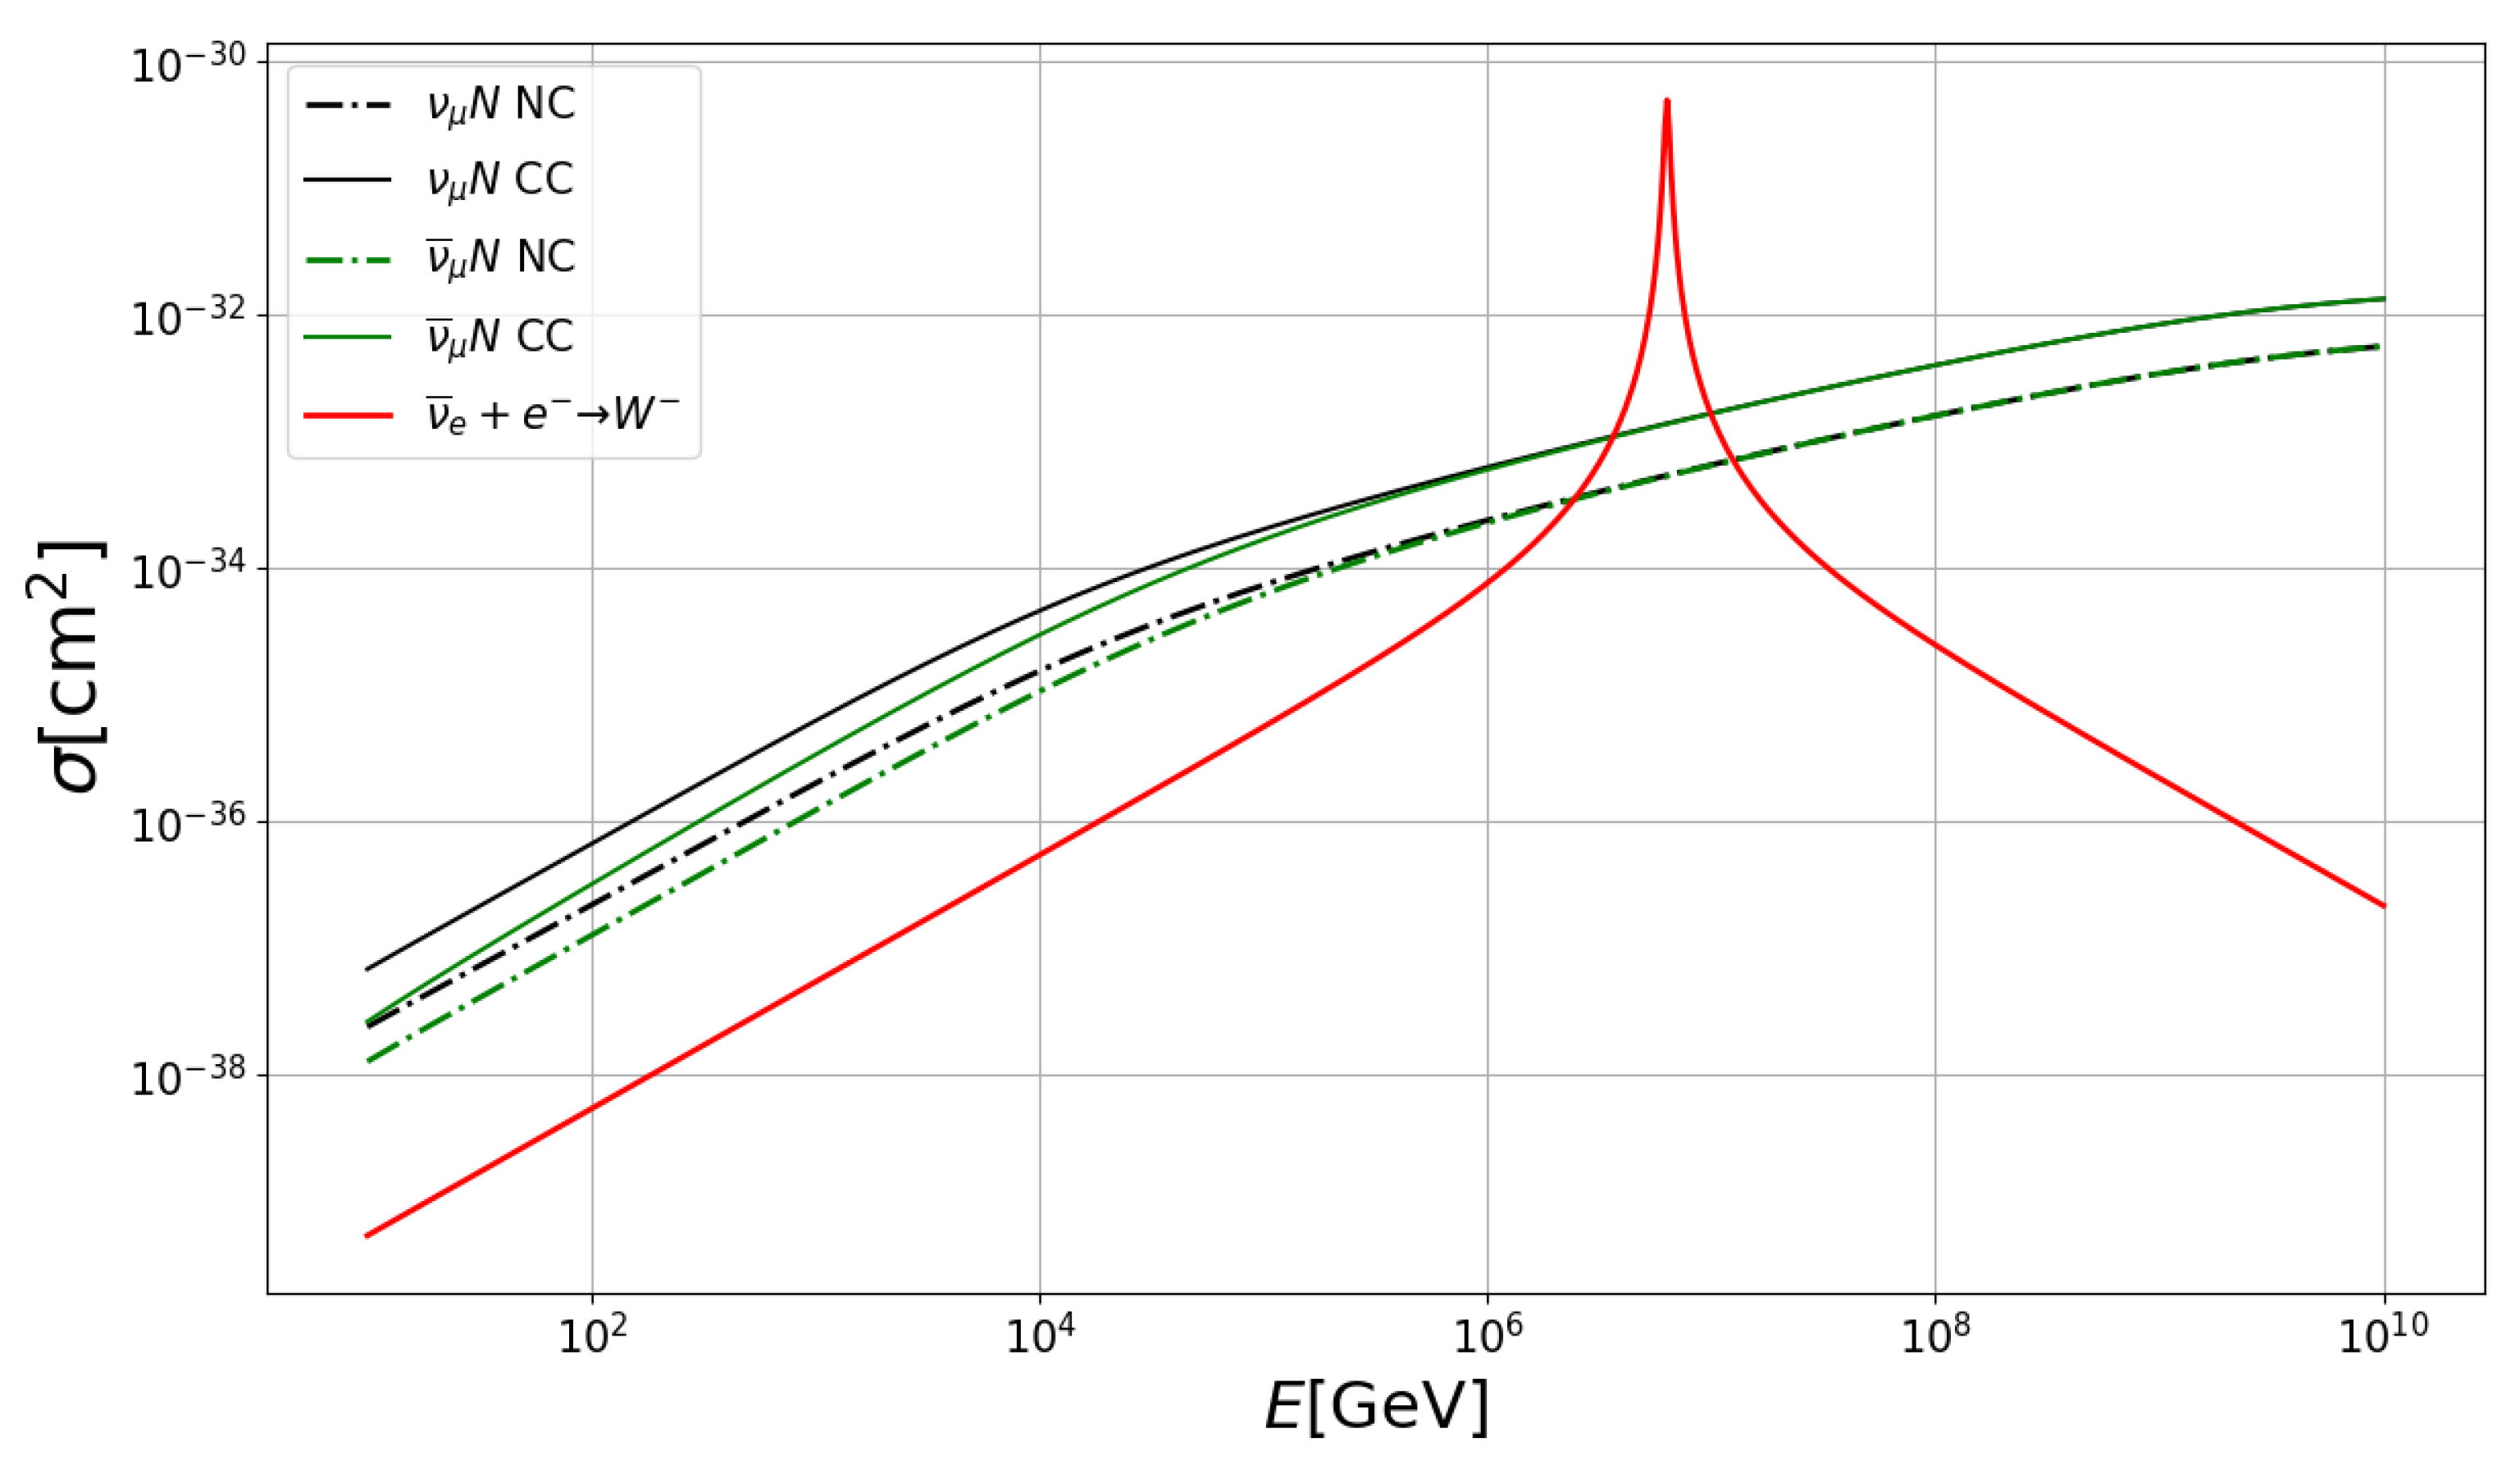
\includegraphics{./figures/nu_phenomenology/xsec_DIS.png}
        \labfig{xsec_DIS}
\end{figure}
A key feature of all structure functions is that they become nearly independent of $Q^2$ in the limit $Q^2 \rightarrow \infty$, meaning cross-section starts to scale linearly with neutrino energy $E_{\nu}$ for up-to $\sim 1$ PeV as shown in \reffig{xsec_DIS}. This property, known as Bjorken scaling, was crucial in developing the parton model for deep inelastic scattering \sidecite{Bjorken_scaling}.  The \reffig{xsec_DIS} illustrates the contributions of CC and NC interactions for both neutrinos and antineutrinos separately. It is evident that the CC cross-section is generally larger than the NC cross-section due to the stronger coupling of the W-boson compared to the Z-boson. At higher energies (> few PeVs), the propagation term from the interaction vertex is no longer dominated by the $W$-$Z$ boson mass. As a result, the cross-section no longer grows linearly with neutrino energy. Moreover, the $(1 - y)^2$ (see second term in bracket of Equation~\ref{eq:DIS_xsec_formula}) suppression that typically allows distinction between neutrino and anti-neutrino interactions is much less pronounced, making the two cross-sections nearly identical \sidecite{Gandhi_1998}.

The calculation of neutrino DIS in the energy range of interest for IceCube has been carried out by Cooper-Sarkar, Mertsch, and Sarkar (CSMS) in 2011 and is the standard that will be used throughout this work to produce neutrino simulation (see Section \ref{sec:mc_sim}) and also to include inelasticity parameter in the forward folding fit (see Section \ref{sec:params}) \sidecite{CSMS}. However, updated cross-section calculations now exists, that takes into account final state radiations (FSR) \cite{xsec_alfonso} and  uses updated parton distribution functions \cite{CT18}. In particular, corrections in visible energy of Glashow events due to FSR were taken into account by introducing a correction in simulation event weight (see Section \ref{sec:glashow_correction} for details). In the last decade, several studies have used different event samples at higher energies to measure the total\footnote{total cross-sections are inclusive of CC and NC interactions.} DIS cross-section in the multi-TeV energy range at IceCube \sidecite{xsec_Sandy, xsec_HESE7}.

\subsubsection*{Glashow Resonance}
\label{sec:glashow}
Neutrinos typically interact with atomic electrons in a detector medium less frequently than with nucleons due to the smaller mass of the electron \sidecite{xsec_overview}. However, an exception occurs during the resonant enhancement of the $\bar{\nu}_e e^-$ scattering cross- section, known as \textbf{the Glashow resonance}. This happens when the center-of-mass energy matches the mass of the $W$-boson. The resonance occurs at an antineutrino energy of $E_{\bar{\nu}} = \frac{M_W^2}{2m_e} \approx 6.3$ PeV, where $m_e$ is the electron mass (see \reffig{xsec_DIS}). Produced W boson, deacays into hadrons/lepton creating a particle shower at around 6 PeV energy. Sheldon Glashow first proposed this phenomenon in 1960 as a method to detect the $W$-boson \sidecite{glashow}. Due to experimental limitations, such high-energy events were not observed for many years. However, the IceCube Neutrino Observatory recently reported detecting a Glashow resonance event, providing the first confirmation of this process \sidecite{glashowic}.

\begin{figure}[h!]
        % \vspace*{4.5cm}
        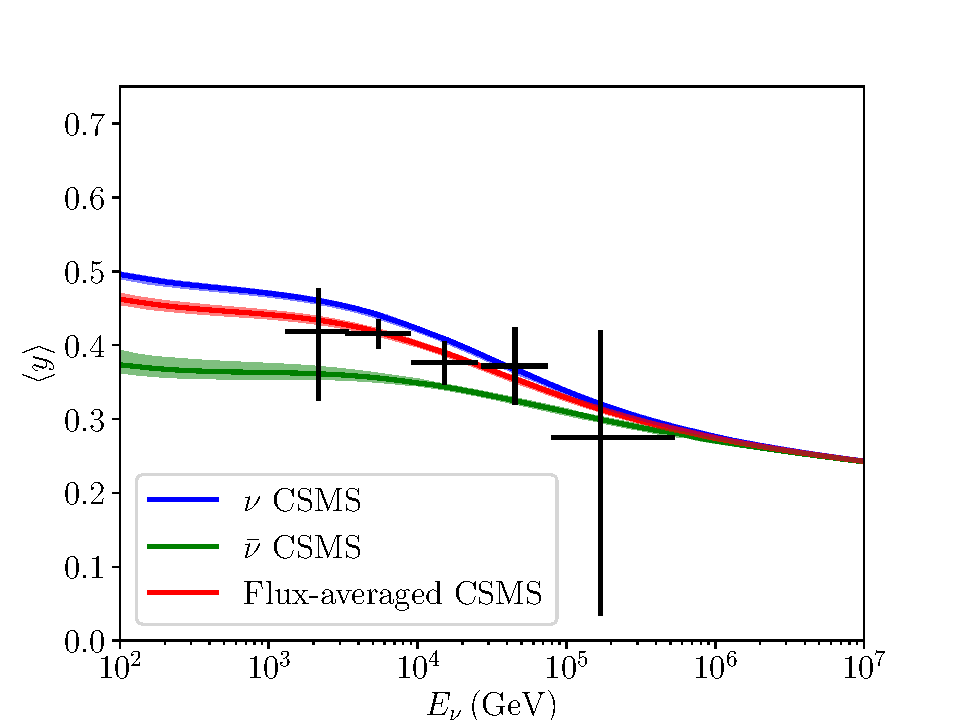
\includegraphics{./figures/nu_phenomenology/split_fit_inel.pdf}
        \caption{The measured mean inelasticity, with error bars indicating 68\% confidence intervals. Predictions from the CSMS model are indicated in blue for $\nu$ and green for $\bar{\nu}$, with theoretical uncertainties shown by the colored bands, along with atmospheric flux-averaged inelasticity in red. Figure taken from \cite{gary_paper}.}
        \labfig{inel_paper}
    \end{figure}

\subsubsection*{Inelasticty}
\label{sec:inelasticity}

Inelasticity, denoted by $y$ as described in Equation \ref{eq:inelasticity}, represents the fraction of the incoming neutrino's energy that is transferred to the hadronic system during deep inelastic scattering (DIS). In neutrino-nucleon DIS, a higher inelasticity corresponds to a larger energy transfer, leading to greater energy deposition in the detector through hadronic showers. Inelasticity can be determined from the kinematics of both the outgoing lepton and the hadronic system. Such a technique was expxloited in an IceCube analysis, to measure inelasticity in TeV range, by using $\nu_{\mu}$-CC events where both interaction vertex (hadronic cascade) and outgoing lepton (\emph{muon track} \sidenote{depending on energy, entire track may or may not be contained within the detector volume, as muon usually deposits some energy along its path and can travel larger distance, possibly leaving the detector, see Section\ref{sec:leptons_inice} for details}) are within the detector \sidecite{gary_paper}. The distinction in inelasticity distribution between $\nu$ and $\bar{\nu}$ (see \reffig{inel_paper}) allows for differentiation between neutrinos and antineutrinos in an event sample. Understanding such an energy dependent inelasticity distribution is crucial for analyzing high-energy neutrino interactions, such as those explored in this thesis, where both hadronic and leptonic energy signatures are used to reconstruct neutrino properties.  


\section{Beyond Standard Model Neutrinos}
\label{sec:bsm}
While the minimum extension used in \ref{sec:nu_mass_osc} provides a framework for describing neutrino oscillations, it also predicts the existence of right-handed neutrinos (or left-handed anti-neutrinos) that do not participate in weak interactions. These non-interacting neutrinos are known as \textbf{\emph{sterile neutrinos}}. Unlike the three active flavors, sterile neutrinos do not contribute to weak interaction processes like $Z^0$ boson decay. Experimental measurements of the $Z^0$ decay width constrain the number of light, active neutrino species (those lighter than the $Z^0$ boson) to 3 \sidecite{Z_decay}. 

Although the three-flavor model is consistent with many observations, anomalies have been observed in several experiments. Radiochemical neutrino experiments \sidecite{radio_chem}, as well as experiments using neutrinos from particle accelerators \sidecite{LSND,MiniBooNE} and anti-neutrinos from nuclear reactors \sidecite{reactor_nu_anamoly}, have reported discrepancies that could be explained by the existence of sterile neutrinos. The simplest theoretical extension to account for these anomalies is the so-called 3+1 model, where one additional sterile neutrino is added to the three active neutrinos. In this model, the PMNS mixing matrix (which describes the mixing between neutrino flavors) is expanded from a $ 3 \times 3$ matrix to a $4 \times 4$ matrix \sidecite{Abazajian:2012ys}. This expanded matrix introduces three new mixing angles ($\theta_{14}, \theta_{24}, \theta_{34} $) and additional CP-violating phases. These additional parameters allow for the mixing of sterile neutrinos with the active ones, potentially explaining the observed experimental anomalies, though further investigation is required to confirm their existence.

Cosmological evidence also provides hints for the existence of sterile neutrinos \sidecite{Abazajian:2017tcc}. The presence of sterile neutrinos could have observable consequences on the evolution of the early universe and on large-scale structure formation. Observations of the cosmic microwave background (CMB) and precise measurements by missions such as WMAP indicate that the number of relativistic species during the early universe, typically expressed as the effective number of neutrino species  $N_{\text{eff}}$, is slightly higher than the expected value of 3 for the three active neutrinos \sidecite{Komatsu_2011}.  This could suggest the presence of additional light particles, such as sterile neutrinos, that contributed to the radiation density in the early universe. Although, another measurement by planck survey is in close agreement with $N_{\text{eff}}=3$ \sidecite{Planck_cosmo}, making the puzzle of such neutrino species even more intriguing.  Moreover, sterile neutrinos could contribute to the dark matter problem \sidecite{kev_dm}. While they are unlikely to account for all dark matter, keV-mass sterile neutrinos are a candidate for \emph{warm dark matter}, a type of dark matter that could impact the formation of structure in the universe on small scales. These cosmological observations, when combined with the experimental anomalies in neutrino oscillation data, make sterile neutrinos an intriguing possibility for both particle physics and cosmology. However, further precision measurements, both in the laboratory and from astrophysical observations, are needed to confirm their existence and determine their exact role in the universe.

In addition to Sterile neutrinos, other exotic phenomena, which are not included in standard model can affect neutrino interaction cross-sections or other fundamental properties assumeed in SM. Such scenarios include interaction of neutrinos with dark matter \sidecite{DarkMatter}, CPT violation \sidecite{CPT_violence} etc. A number of analysis have been made in IceCube to look for sterile neutrinos \sidecite{Trettin2024Search}, other exotic neutral leptons \sidecite{Fischer2024First} and also to look for dark matter signatures \sidecite{IceCube:2023ies} have been made. Although, as it will be discussed in the next chapter, for the analysis presneted in this thesis, as none of these scenraios, when probed to measure flavour fraction of astrophysical neutrinos on earth allows for non-zero tau neutrino fraction \sidecite{overview_bsm_flavour}, hence they are not discussed further in detail, and for the remainder of this thesis, 3 flavour of neutrinos shall be assumed. 